%--------------------------------------------------------------------------------------------------------------------
% This replicates (with some cleaning), in tikz, the diagrams from Leo Breiman's famous
% 2001 paper:
% @article{breiman2001,
% 	author = {Breiman, Leo},
% 	title = {Statistical modeling: The two cultures (with comments and a rejoinder by the author)},
% 	journal = {Statistical Science},
% 	volume = {16},
% 	number = {3},
% 	year = {2001},
% 	month = aug,
% 	pages = {199-231},
% 	doi = {10.1214/ss/1009213726}
% }
% Replicated by Momin M. Malik, September 2022
%--------------------------------------------------------------------------------------------------------------------


\documentclass[border=10pt, crop, varwidth]{standalone} 
\usepackage{tikz}

\usetikzlibrary{chains}
\usetikzlibrary{arrows}

\begin{document}

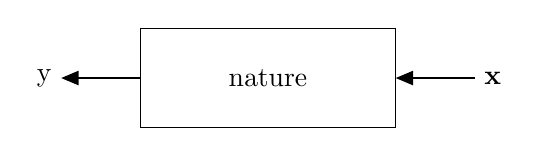
\begin{tikzpicture}

  % Define nodes
  \node[draw, rectangle, pos=.5, text width=3cm, align=center, minimum height=3*\baselineskip] (nature) {nature};
  \node[left=of nature] (y) {$\textrm{y}$};
  \node[right=of nature] (x) {$\textbf{x}$};

  % Connect the nodes
  \draw [->, >={triangle 45}] (x) -- (nature);
  \draw [->, >={triangle 45}] (nature) -- (y);

\end{tikzpicture}

\vspace{3em}

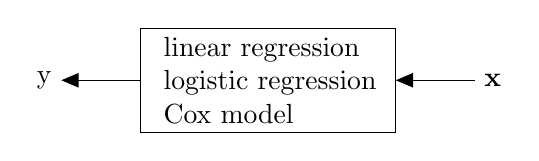
\begin{tikzpicture}

  % Define nodes
  \node[draw, rectangle, pos=.5, text width=3cm, align=left, minimum height=1em] (nature) {\,~linear regression\\\,~logistic regression\\\,~Cox model};
  \node[left=of nature] (y) {$\textrm{y}$};
  \node[right=of nature] (x) {$\textbf{x}$};

  % Connect the nodes
  \draw [->, >={triangle 45}] (x) -- (nature);
  \draw [->, >={triangle 45}] (nature) -- (y);

\end{tikzpicture}

\vspace{3em}

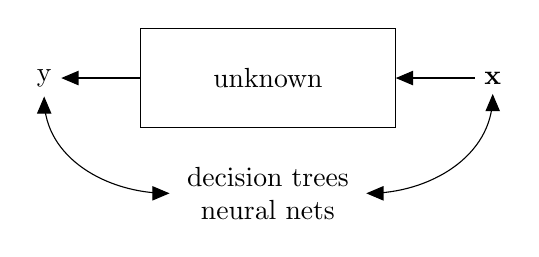
\begin{tikzpicture}

  % Define nodes
  \node[draw, rectangle, pos=.5, text width=3cm, align=center, minimum height=3*\baselineskip] (unknown) {unknown};
  \node[left=of unknown] (y) {$\textrm{y}$};
  \node[right=of unknown] (x) {$\textbf{x}$};
  \node[below=of unknown, yshift=1.5\baselineskip, text width=2.25cm, align=center] (ml) {decision trees\\neural nets};

  % Connect the nodes
  \draw [->, >={triangle 45}] (x) -- (unknown);
  \draw [->, >={triangle 45}] (unknown) -- (y);
  \draw [<->, >={triangle 45}] (y.south) to [out=270,in=180] (ml.west);
  \draw [<->, >={triangle 45}] (ml.east) to [out=0,in=270] (x.south);

\end{tikzpicture}

\end{document}